\epigraph{\textit{If you don’t believe it or don’t get it, I don’t have the time to try to convince you, sorry.}}{––\textsc{Satoshi Nakamoto}, Founder of Bitcoin}

\section{Introduction}
In this chapter we extend our analysis of interest rate swaps to consider the case within cryptocurrency markets. We begin with a discussion of the terminology and existing products before reviewing traditional interest rate models, examining a proposed crypto interest rate model and constructing some indicative yield curves. We then consider a specific crypto interest rate swap: the Bitcoin-USD Funding Rate Swap, its mechanics and pricing formula. We finish by briefly proposing some new areas for interest rate swap-like products within crypto markets. 

\section{Terminology \& Products}
The world of cryptoassets is considerably different to that of traditional finance. It represents a new approach towards storing and transacting value, based on new technologies. This difference introduces new terminology that, once again, must be understood in order to fully appreciate the products on offer. Some elements have close ties with traditional counterparts, just with different names, whilst others are completely new.

Given the decentralised nature of cryptocurrencies, a mechanism is required to solve the so-called `double spending' problem––that is, some way of ensuring one cannot spend the same money twice. In traditional finance there would simply be a central authority, such as a central bank, responsible for keeping track of such issues but in crypto there is no such thing. To solve this challenge, and give cryptocurrencies credibility and inherent value, two approaches have since been used: \textit{Proof-of-Work} and \textit{Proof-of-Stake}.

\subsection{Proof-of-Work (PoW)}
The proof-of-work technique relies on miners seeking to be the first to solve a cryptographic puzzle. The first miner to do so then adds the next block to the blockchain and is rewarded with a specified amount of cryptocurrency. The challenge arises from the complexity of the cryptographic puzzle itself, as solving such a problem requires enormous amounts of computational power (and has since been criticized for its energy inefficiency). Although given the sheer number of participating miners around the world, it only takes an average of ten minutes to solve \citep{balan2021long}. The technique can be considered self-regulating since each miner has an incentive to be the first to provide the correct answer and be the one to update the blockchain, thereby earning the reward. The open source nature of the protocol means an incorrect answer, submitted by a miner in a bid to earn the reward, would easily be identified by other participants and would be rejected \citep{crypto_pow}. 

\subsection{Proof-of-Stake (PoS)}
The proof-of-stake technique proposes an alternative to proof-of-work. The method relies on participants contributing, or \textit{staking}, their cryptocurrency for the chance to become a validator, add the next block to the blockchain, and subsequently be rewarded with a specified amount of cryptocurrency. Unlike proof-of-work, this is not a race. The selection of the validators depends on how much cryptocurrency is staked and the length of time it has been staked for. Those who have been selected as validators confirm that the block is correct and other participants (those not initially selected) can review and attest to the correctness of that block. If there are no issues, then the selected validators earn a reward. With proof-of-stake, however, the self-regulation stems from consequences of an incorrect block. If the non-selected validators disagree, and prove the proposed block to be incorrect, then the initial validators will lose some of their staked cryptocurrency in a move known as \textit{slashing} \citep{crypto_pos}.

\subsection{Staking}
Whilst the proof-of-stake mechanism is conceptually simple, the actual investment required to become a potential validator can be substantial, not to mention requiring a large amount of computational resources and an in depth understanding of the fundamental technology. This often puts it out of reach for moderate investors. 

To reduce the barriers to entry, crypto exchanges now offer staking as a product to their clients. This means that smaller investors can contribute their cryptocurrency into a pool which is then used participate in the proof-of-stake mechanism, and earn crypto `interest' in return. This often requires some lock-up period, in which contributors to the pool will not have access to their assets, with any withdrawal attempts triggering significant penalties. The approach is very similar to, say, a traditional US Treasury bond fund––few investors could buy the bonds outright, but any investor can purchase a bond fund and earn their share of interest (coupon payments) through participation. 

Given the high volatility in crypto markets, this product poses serious risks. If the price of the cryptocurrency staked drops over the lock-up period, then it is possible that the loss on the underlying will outweigh the interest earned over the period. This widespread problem is referred to as the \textit{impermanent loss} and is felt by many participants, including market makers \citep{crypto_staking}.

\subsection{Crypto Saving \& Lending}
Staking should not be confused with crypto \textit{savings products}. As with traditional finance, it is possible to deposit cryptocurrency into a savings account, offered by crypto exchanges, and earn interest in the form of crypto on that deposit. One has the option of locked or flexible savings accounts, with flexible providing instant access and locked only being available for withdrawal after a specified time period, as expected \citep{crypto_saving}.

A \textit{crypto loan} is somewhat analogous to a traditional loan in that it refers to the borrowing of funds over a specific time period with an agreement to repay the loan with interest. The difference, however, is that in the majority of cases the funds being borrowed are cryptocurrencies, and the collateral is another cryptocurrency. It is worth noting that this is not always the case, as firms like Celsius (prior to filing for bankruptcy) offered USD loans, with collateral of cryptocurrency \citep{celsius}. 

To protect themselves, firms offering these products often require overcollateralisation, that is, the value of the cryptocurrency secured against the loan is significantly more than the loan itself. In addition, there are aggressive margin requirements that require further collateral deposits should the markets move negatively, with a threshold at which the company has the right to sell the secured cryptocurrency and close the loan. Once again, given the high volatility in crypto markets, the products pose serious risks \citep{crypto_loan}.

\subsection{Crypto Swaps}
Due to its early divergence from traditional finance, the term \textit{crypto swap} already has meaning, hence, we must be explicit when discussing forthcoming \textit{crypto interest rate swaps}. A crypto swap refers to the direct swap of one cryptocurrency for another and is analogous to an FX swap. In general, there are two methods for doing so. Firstly, one can use a centralised crypto exchange, however, this leads to certain unwanted characteristics, such as the power the exchange has over any transaction. They could limit the available cryptocurrencies or charge a fee for their services. The second method involves a trustless exchange using the atomic swap protocol which utilises a specific type of cryptographic holding period called Hashed Time Lock Contracts \citep{liu2020atomic}.

\subsection{Liquidity Pooling}
Of course, pursuing a crypto swap through an exchange requires there to be sufficient demand for each of the tokens in question, such that the exchange can offer the desired swaps. To establish a broader range of swap pairs, exchanges set up liquidity pools. These are essentially large collections of tokens that enable parties to swap their cryptocurrencies. To increase the size of the collection––since a larger pool equates to a more liquid swap pair––individuals can contribute their own cryptocurrencies to one, or both, sides of the pair (provided they own those assets prescribed by the swap pair). As a result, they are rewarded by earning a `portion' of the returns on the transactions that occur.

The level of risk is primarily determined by the swap pair itself. For more stable tokens the lower volatility can lead to more predictable returns, albeit they are generally smaller. Alternatively, for pairs of which one, or both, are not stable tokens market volatility plays a much larger role and the returns are subject to greater variation, perhaps even resulting in losses.

\section{Crypto Interest Rates}

In the case of traditional markets, the concept of interest is simply one that rewards existing holders of assets. The idea that one can deposit their assets for a specific period of time after which they will receive slightly more than they previously held. This extends throughout the traditional finance system and is not limited to individuals; generic companies can deposit cash or other marketable instruments with financial institutions to earn interest, and likewise financial institutions themselves can make deposits to central banks. This has fueled the development of the numerous short rate models over the years, and is fundamental to derivatives pricing. 

This is contradictory, however, to the world of cryptocurrencies. It is not the owners of cryptoassets that are rewarded, but the miners in a proof-of-work protocol and the validators in the proof-of-stake case. In addition, the decentralised nature of crypto means there is no central bank or authority by definition. This implies that the short rate is zero. How, then, can one construct a non-trival interest rate term structure model? Before examining the model itself, it will be useful to review the traditional case.

\subsection{Traditional Interest Rate Models}
The development of traditional short rate models begins with the assumption of the probability triple $(\Omega, \mathcal{F}, \mathbb{P})$, where $\{\mathcal{F}\}_{s \geq 0}$ is the associated filtration. We then proceed to define the adapted short rate process $\{r_s\}_{s \geq 0}$. 

Recall from definition \ref{disc_fact} the idea of a discount factor, $Z(0,t_i)$, the present value of \$1 received at some point, $t_i$, in the future. We briefly mentioned the fact that this was equivalent to the price today of a zero coupon bond, with a principal of \$1, maturing at time $t_i$, before proceeding to demonstrate its links to spot rates and forward rates.

We can define this discount factor, or zero coupon bond, more generally using the short rate process, $r_s$ instead. Let $\mathbb{Q}$ be an appropriate risk-neutral measure equivalent to our initial measure $\mathbb{P}$, and $0 \leq s < t_i$ be any time prior to maturity, then we can write

\begin{equation}
\label{zcb_expectation}
    Z(s, t_i) = \mathbb{E}^{\mathbb{Q}} \left[ \exp \left( - \int_{s}^{t_i} r_u du \right) \bigg \vert \mathcal{F}_s \right].
\end{equation}

As it so happens, the representation given in \ref{zcb_expectation} is not the only one possible. \cite{constantinides1992theory} introduced a new approach to interest rate modelling using \textit{pricing kernels}. A pricing kernel is an $\mathcal{F}_s$-adapted càdlàg semimartingale $\{ \pi_s \}_{s \geq 0}$ satisfying certain conditions. This leads to an alternative, but equivalent, representation of our zero coupon bond

\begin{equation}
\label{zcb_alt}
    Z(s,t_i) = \frac{1}{\pi_s} \mathbb{E} \left[ \pi_{t_i} \vert \mathcal{F}_s \right].
\end{equation}

We can quickly recover the expression \ref{zcb_expectation} as follows. Using the money market account as our numeraire, given by

\begin{equation}
    B_s = \exp \left( \int_0^s r_u du \right)
\end{equation}
we have that the combination of the inverse of the money market account (that is, discounting) and the Radon-Nikodym derivative forms our pricing kernel,

\begin{equation}
    \pi_s = \exp \left( -\int_0^s r_u du \right) \frac{d \mathbb{Q}}{d \mathbb{P}} \bigg \vert_{\mathcal{F}_s}.
\end{equation}

As a result, we can use the typical change of measure technique on \ref{zcb_alt} to obtain our original expression. For more information regarding risk-neutrality, change of measure, and change of numeraire, the reader is referred to the excellent discussion in Chapter 2 of \cite{brigo2001interest}.

\subsection{A Crypto Interest Rate Model}
Regardless of the approach used, it is difficult to imagine the circumstances under which we can produce a non-trivial term structure given an identically zero short rate ($r_u = 0$). In addition, our previous comments on the concept of traditional versus decentralised `interest' excludes any reliance on the money market account, since there will be no growth in cryptoassets held, that is, the process $B_s$ is constant.

To produce a non-trivial term structure model, \cite{brody2020theory} relies on choosing a pricing kernel that is a strict local martingale, which produces the desired effect of a zero short rate. The pricing kernel in question is the reciprocal of a Bessel(3) process (this is later extended to consider Bessel($n$) processes, however, we will omit this generalisation from our work). 

Assume the existence of a probability triple ($\Omega$, $\mathcal{F}$, $\mathbb{P}$), with adapted filtration $\{\mathcal{F}_s \}_{s \geq 0}$. Further, define three standard, independent Brownian motions $\{W_s^{(1)}, W_s^{(2)}, W_s^{(3)}\}_{s \geq 0}$ and let $\sigma_s$ be a bounded, strictly positive deterministic function. Then

\begin{align}
    X_s &= \int_0^s \sigma_u dW_u^{(1)} \\
    Y_s &= \int_0^s \sigma_u dW_u^{(2)} \\
    Z_s &= \int_0^s \sigma_u dW_u^{(3)}
\end{align}
and our pricing kernel, the reciprocal of a Bessel(3) process, is given by
\begin{equation}
    \pi_s = \frac{1}{\sqrt{(X_s - a)^2 + (Y_s - b)^2 + (Z_s - c)^2}}
\end{equation}
where $a, b, c \neq 0$. We also require the initial condition $\pi_0 = 1$, hence, we must have that $\sqrt{a^2 + b^2 + c^2} = 1$.

Now, using equation \ref{zcb_alt} we find,

\begin{equation}
    Z(s,t_i) = \frac{1}{\pi_s} \mathbb{E} \left[ \frac{1}{\sqrt{(X_{t_i} - a)^2 + (Y_{t_i} - b)^2 + (Z_{t_i} - c)^2}} \bigg \vert \mathcal{F}_s \right].
\end{equation}

At this point we can rely on the definition of Brownian motion and observe that $X_{t_i} - a = (X_{t_i} - X_s) + (X_s - a)$, similarly for $Y_{t_i}$ and $Z_{t_i}$. Hence, we find that

\begin{align}
    X_{t_i} &\sim \mathcal{N}(X_s - a, \Sigma_{s,t_i}) \\
    Y_{t_i} &\sim \mathcal{N}(Y_s - b, \Sigma_{s,t_i}) \\
    Z_{t_i} &\sim \mathcal{N}(Z_s - c, \Sigma_{s,t_i}) \\
    \Sigma_{s,t_i} &= \int_s^{t_i} \sigma_u^2 du.
\end{align}

After a great deal of algebra, \cite{brody2020theory} arrives at the expression for the zero coupon bond price. Given by,

\begin{equation}
    Z(s,t_i) = \text{erf} \left( \sqrt{ \frac{(X_s - a)^2 + (Y_s - b)^2 + (Z_s - c)^2}{2 \Sigma_{s,t_i}}} \right)
\end{equation}
where erf($\cdot$) is the standard error function defined as,
\begin{equation}
    \text{erf}(z) := \frac{1}{\sqrt{\pi}} \int_{-z}^{z} e^{-u^2} du.
\end{equation}

Now that we have an explicit formula for the price of zero coupon bond, we can use the following relation to compute the yield curve \citep{wilmott2013paul}

\begin{equation}
    Y(s,t_i) = -\frac{1}{(t_i - s)} \log Z(s, t_i).
\end{equation}

Thus we obtain the explicit expression, for $s = 0$

\begin{equation}
\label{crypto_yield}
    Y(0,t_i) = -\frac{1}{t_i} \log \left[ \text{erf} \left(\frac{1}{ \sqrt{2 \Sigma_{0,t_i}}} \right) \right].
\end{equation}

\subsection{Crypto Yield Curves}
From \ref{crypto_yield} we have a closed form expression for the yield curve provided we can appropriately identify $\Sigma_{s,t_i}$, or more specifically $\sigma_u$ underlying it. Using a constant value for volatility, similarly to \cite{brody2020theory}, we can produce some illustrative yield curves displayed in Figure \ref{fig:crypto_yield}.

\begin{figure}[ht]
\begin{center}
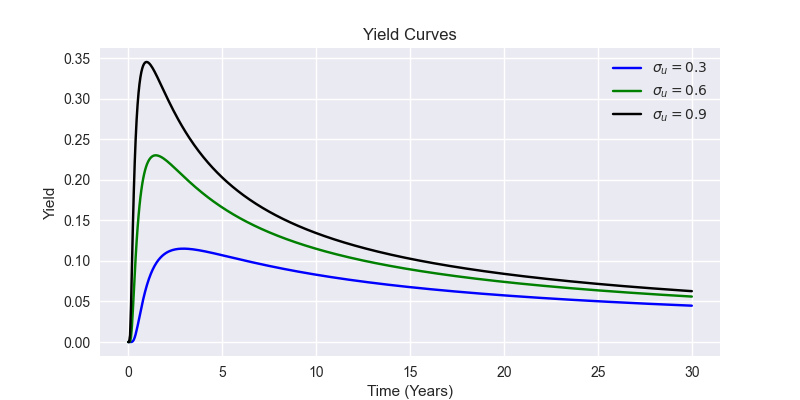
\includegraphics[width=0.99\textwidth]{Chapter_4/images/crypto_yield.png}
\caption[Indicative Crypto Yield Curves]{Examples of a crypto yield curve based on constant values of $\sigma_u$. Reproduced from \cite{brody2020theory}.}
\label{fig:crypto_yield}
\end{center}
\end{figure}

In practice, we would be more likely to work in the opposite direction. We would use the explicit formula for the yield curve to calibrate our volatility function $\sigma_u$ to market data, just as one can compute implied volatility from the original \cite{black1973pricing} solution using an iterative technique.

\section{Crypto Interest Rate Swaps}
Cryptocurrency interest rate models are still in their infancy and there is yet to be a widely recognised and agreed upon approach. The intention, however, has led some crypto market participants to offer an early foray into the world of interest rate derivatives, and specifically interest rate swaps.

As discussed in Chapter 3, interest rate swaps are model independent, by which we mean that they sidestep the challenges faced by the lack of established crypto interest rate models. A general fixed-for-floating interest rate swap simply exchanges a series of fixed interest rate payments for a series of floating ones, but there are no restrictions on what the `interest rate' is. This makes it a prime candidate to be extended to crypto markets provided there exists a product that, one way or another, involves variable payments. 

The cryptocurrency exchange BitMEX offers one such product: \textit{perpetual swaps} (recall, in this instance we are referring to swaps in the crypto sense––the exchange of one asset for another––similar to traditional currency exchange). Let us first understand one specific example of BitMEX's perpetual swaps, the Bitcoin-USD (`XBTUSD') perpetual swap, before considering its associated interest rate swap.

\subsection{Bitmex XBTUSD Perpetual Swap}
A perpetual swap behaves similarly to a traditional futures contract, however, as the name suggests, there is no contract settlement date. The XBTUSD contract specifically is an \textit{inverse} contract, that is, the opening and closing prices are the reciprocal of the quoted XBTUSD conversion rate. In mathematical terms, this means the profit or loss to the long party is calculated as

\begin{equation}
    \text{Profit/Loss} = \text{No. of Contracts} \times \$1 \times \left(  \frac{1}{\text{XBTUSD}_{open}} - \frac{1}{\text{XBTUSD}_{close}}\right)
\end{equation}
where the \$1 reflects the multiplier for the contract.

As with traditional futures, the contracts are marked-to-market daily, although in crypto this process is called \textit{fair price marking}, and initial and maintenance margin are required in tandem with traditional derivatives exchanges.

Whilst the XBTUSD contract is perpetual, holding the contract (either long or short) still requires a form of `rolling over'. This occurs via a \textit{funding rate}, which is either paid or received depending on the computed rate and the direction of the position held, calculated every 8 hours. 

The actual calculation of the funding rate is non trivial and is beyond the scope of this project. Nevertheless, it is important to note some of its features.

\begin{itemize}
    \item The amount paid is calculated upon the notional value of the contract, rather than the margin position, hence is independent of leverage;
    \item The XBTUSD funding rate consists of three components: the interest rate, the discount or premium, and a dampening element;
    \item The interest differential is determined using the prevailing XBT and USD lending rates, divided by the number of funding periods per day (in this case three);
    \item The funding rate is then calculated every minute over the period and a time-weighted average price is applied. This determines the funding rate for the next period, that is, the funding rate is always known eight hours in advance.
\end{itemize}
In general, the funding rate is positive and long parties pay the funding rate, while short parties receive.

\subsection{Bitmex Funding Rate Swap}
The variability of the funding rate is analogous to the floating rate exposure associated with traditional markets discussed in Chapter 3––consider a borrower with an outstanding loan tied to LIBOR rates. This means parties involved in XBTUSD perpetual swaps may naturally look towards derivatives contracts to hedge the uncertainty of future funding rates.

The BitMEX Funding Rate Swap, offered by the Singapore based Delta Exchange, precisely filled that gap. Functioning in a similar way to a general fixed-for-floating interest rate swap in traditional markets, the funding rate swap is an agreement to exchange a fixed rate payment for a series of floating rate payments tied to the funding rate of the BitMEX XBTUSD perpetual swap, thus swapping the floating rate for a fixed rate exposure. 

It is worth noting that the funding rate swap is similar, but not identical, to traditional interest rate swaps since there is a lump sum payment associated with fixed rate side at the initiation of the contract, while the floating payments are paid in series. 

Furthermore, under normal circumstances when the funding rate is positive and long parties compensate short parties, the long party entering into a funding rate swap is said to be \textit{buying floating-for-fixed}. This means they are paying a fixed rate and receiving a floating rate (this would be deemed a \textit{payer swap} in traditional terms). On the contrary, the short party entering into a funding rate swap is said to be \textit{selling floating-for-fixed}, by which we mean they are receiving a fixed rate and paying the floating funding rate (a \textit{receiver swap} in traditional terms). 

\section{Pricing a Bitmex Funding Rate Swap}

\subsection{The Pricing Formula}
In traditional markets we observed that the `price' of a general fixed-for-floating interest rate swap was simply the fixed rate quoted on an annualised basis. This is somewhat the case in decentralised markets, as the prices observed in the orderbook are the fixed rates associated with the contracts, again quoted on an annualised basis.

However, since the payment related to the fixed leg of the contract is paid immediately at the start of the contract, it holds closer ties to the concept of a \textit{premium} in option pricing, and as such holds the same name. This premium represents a cash outflow for those buying floating-for-fixed, whilst the opposite is true for those selling. 

In a similar manner to traditional fixed-for-floating interest rate swaps, we can consider the fixed rate of the BitMEX Funding Rate Swap as being determined by market forces––Delta Exchange's orderbook contains bids and offers, submitted by market participants, of annualised fixed rates. This means we are concerned with computing the premium of the contract.

Let $r_s$ be the fixed rate of the funding rate swap. Given the increased frequency of funding periods, every eight hours, the premium is calculated using the time to maturity in seconds. To emphasise this point, we will denote the time to maturity as $\bar{\tau}$. Then the premium can be calculated as

\begin{equation}
\label{irs_premium}
    \text{Premium} = \text{Notional} \times r_s \left( \frac{1}{\text{XBTUSD}} \right) \left( \frac{\bar{\tau}}{31536000} \right)
\end{equation}
where the 31,536,000 is the number of seconds in a year. The notional principal merely acts as a scaling factor, although given the price of XBTUSD (around \$21,500 at time of writing) and the fact that the XBTUSD perpetual swap is an inverse contract, it will be important in the forthcoming numerical example to ensure the calculations remain at an appropriate scale.

\subsection{Numerical Example}

To firmly cement our understanding of the mechanics and calculations associated with the BitMEX Funding Rate Swap we will consider a numerical example. In an effort not to overcomplicate the scenario, we will make the following assumptions:

\begin{enumerate}
    \item The price of XBTUSD remains constant throughout the life of the funding rate swap. This prevents us from needing the true spot rate at the time of each funding period in order to convert the USD denominated floating rate payments into XBT;
    \newpage
    \item The funding rate remains constant throughout the life of the contract. Of course, the future funding rates would be unknown by definition, however, this allows us to illustrate the balancing of fixed and floating payments;
    \item We will consider the example from the perspective of the long party under normal circumstances––that is, the funding rate is positive;
    \item The fixed rate is determined by supply and demand. 
\end{enumerate}
Our input data is as follows.

\begin{table}[ht]
\begin{center}
\begin{tabular}{lc}

\toprule
\multicolumn{2}{c}{\textit{BitMEX XBTUSD Funding Rate Swap}} \\
\toprule
\multicolumn{2}{c}{\textsc{Contract Details}} \\
\toprule

Notional & \$100,000 \\
XBTUSD Spot & \$21,500 \\
Fixed Rate (p.a.) & 17\% \\
Funding Rate (8h) & 0.015\% \\
Funding Rate (p.a.) & 16.425\% \\
Time to maturity (days) & 90 \\
Time to maturity (seconds) & 7,776,000 \\
\toprule

\end{tabular}
\end{center}
\caption[BitMEX XBTUSD Perpetual Funding Rate Swap––Contract Details]{The observed market data used as inputs for the funding rate swap numerical example.}
\label{tab:xbtusd_irs}
\end{table}

\subsubsection{The Fixed Rate Leg (Upfront Premium)}

The fixed rate leg requires upfront payment of the premium using \ref{irs_premium}

\begin{align}
    \text{Premium} &= \text{100,000} \times 0.17 \left( \frac{1}{\text{21,500}} \right) \left( \frac{7,776,000}{31,536,000} \right) \\
    &= 0.19496655.
\end{align}
This value is denominated in XBT and must therefore be converted using the spot rate and quoted in USD in line with the terms of the contract. Therefore,
\begin{equation}
    \text{Premium} = \$4191.78.
\end{equation}

\subsubsection{The Floating Rate Leg}

In practice, we would not be able to compute the amount paid by the floating leg until the maturity of the contract. For our purposes, however, we have assumed a constant funding rate to illustrate the concept. 

The floating leg is required to pay the funding rate every eight hours. At three funding periods per day for 90 days we have a total of 270 payment frequencies. In addition, we observed that the funding rate was 0.015\%. Thus we have that,

\begin{align}
    \text{Total Payment} &= \text{Notional} \times \text{No. of Periods} \times \text{Funding Rate} \\
    &= 100,000 \times 270 \times 0.00015 \\
    &= \$4050.
\end{align}

\subsubsection{Discussion}
As we can see the two payments are similar but not equal. The willingness by the long party to pay an annualised fixed rate of 17\% suggests that they believe the funding rate will increase during the life of the contract. They could simply be speculating with the sole aim of earning a profit should their view be correct, or they could be seeking to manage their risk. This would likely be the case if they held an existing position in the underlying BitMEX XBTUSD Perpetual Swap, with a long term strategic view and wanted to reduce the uncertainty of future funding rates. 

Of course, if one truly did believe that the funding rate would remain constant during the life of the contract, then the fair price would be that which has a value of zero at initiation, just as with traditional interest rate swaps. In our example, the fixed rate would be quoted as 16.425\%––identical to the annualised funding rate––and the premium would be precisely \$4050. This observation puts forward a strong case for the further development of cryptocurrency interest rate models, applied directly to the funding rate of perpetual contracts. 

\section{Extensions to Alternative Cryptocurrencies}

\subsection{DAI Savings Rate Swap}
As mentioned, the availability of interest rate swap-like products within the the crypto market is sparse. We focused on one of only two which have clear documentation, the XBTUSD Funding Rate Swap, with the other being the DAI Savings Rate Swap.

As the name suggests, the product is an agreement to swap the variable rates earned for depositing collateral into the DAI `vault' for a fixed rate. The mechanics are almost identical to that of the XBTUSD Funding Rate Swap in that the premium associated with the fixed leg is paid at initiation of the contract, and the fixed rate is determined by market forces. We will omit the details, although it is worth noting there is no underlying inverse contract, hence, the premium is a simple multiplication. 

\subsection{Further Generalisations}

Both the XBTUSD Funding Rate Swap and Dai Savings Rate Swap provide excellent blueprints for further generalisations to other crypto offerings. We now present some potential avenues within the crypto market which could offer interest rate swap-like products.

\subsubsection{Other Perpetual Swap Contracts}
The BitMEX XBTUSD Funding Rate Swap relies on the perpetual nature of the underlying and the fact it has an associated funding rate as the contract is `rolled over'. This practice, however, is not exclusive to this currency pair. In fact, there are plenty of other perpetual swap contracts citing different currencies, some of which continue to act as a bridge between traditional fiat currencies and cryptocurrencies, while others are pure crypto pairs. Regardless, each contract has its own associated funding rate and therefore the same principal can be applied.

Consider, for instance, the ETHUSD Perpetual Swap. Other than the name of the token, there is virtually no mechanical difference between an XBTUSD funding rate swap and an ETHUSD funding rate swap. Excluding external factors such as the demand and economic cost of offering such a product, there is clearly a theoretical basis for the extension of the specific funding rate swap previously discussed to cover more general currency pairs. 

\subsubsection{Staking}
Staking has become a popular option for crypto investors to earn a yield on their assets by contributing them to a proof-of-stake mechanism and being rewarded for doing so. The lockup period can range from 10–120 days at which point the yield earned on the stake (quoted on an annualised basis) may have changed.

It is conceivable then that those looking to continuously stake their assets for an extended period of time may be willing to exchange the uncertain future staking yields for a stream of known fixed interest payments. Consider the following example.

The token `UCL' functions using a proof-of-stake mechanism. An investor holding UCL tokens is bullish about its future prospects and believes its value will rise one year from now. He or she is therefore unwilling to sell their position, but wishes to maximise returns over this period.

The investor decides to contribute their UCL tokens to a staking pool, which has a lockup period of 30 days, after which they will receive their staked position and the associated interest payment, before recommitting the same position to the staking pool. At each rollover date, there is uncertainty surrounding the staking yield offered.

As a result, the investor enters into a contract––for which we will coin the term \textit{Staking Yield Swap}––in which they agree to pay the variable rate of interest earned on their staked investment every 30 days and receive a fixed rate. By definition such an arrangement could be considered an interest rate swap-like product. 

\subsubsection{Crypto Saving \& Lending}
The concept of the Dai Savings Rate Swap could easily be applied to any crypto savings products that pay a variable rate of interest. In principal this is very similar to the Staking Yield Swap defined above since an investor is essentially depositing their investment and receiving interest, however, savings products may allow for more flexibility in terms of redemption. Once again, there are currently no other products besides the Dai Savings Rate Swap but there is sound theoretical basis for extension to general \textit{Savings Rate Swaps}.

The increasing prevalence of crypto lending offers an opportunity for interest rate swaps to be used analogously to traditional markets. That is, a company offering floating rate crypto loans can hedge their risk by entering into what we might deem a plain vanilla pay floating receive fixed \textit{crypto interest rate swap}. At present no such products exist. Of course, this precludes the challenges crypto loan platforms have faced with recent market volatility and wider bankruptcies.

\subsubsection{Liquidity Pooling}
Our final consideration is liquidity pooling in which depositing one, or both, cryptocurrencies into a pool allows investors to earn a variable yield. Given the previous extensions it is clear that we can once more imagine a scenario in which an investor wishes to swap the variable floating yield received from the pool for a fixed rate and, hence, we coin the term \textit{Liquidity Yield Swap}. As before, no such products currently exist.
